% The plots are the committed PNGs. Committing vector PDFs needs an exception in .gitignore,
% which excludes *.pdf; results/estimator-variance/summary.csv holds the plotted values.
\todo[inline]{TODO: replace the PNG plots below by vector PDFs before submission.}

\begin{figure}[H]
    \centering
    \begin{subfigure}[t]{0.32\linewidth}
        \centering
        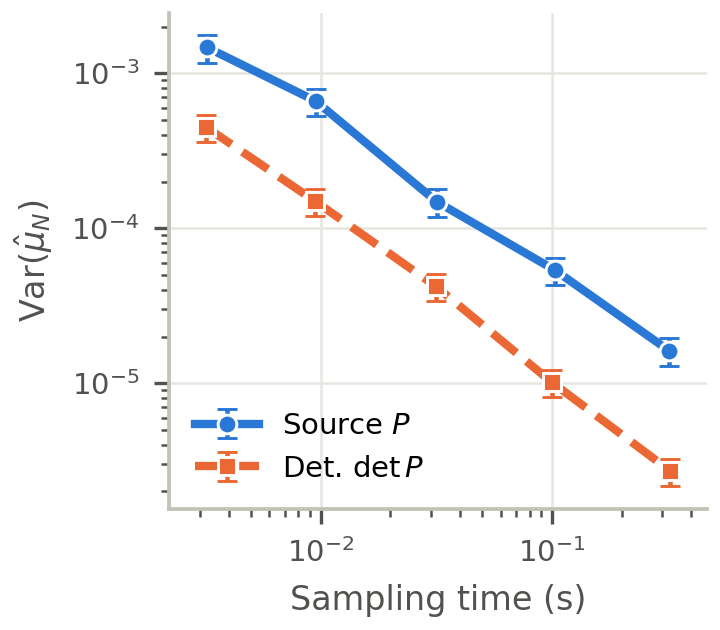
\includegraphics[width=\linewidth]{../results/estimator-variance/branching.png}
        \caption{\texttt{branching}: $6.0\times$ lower}
        \label{fig:estimator-variance-branching}
    \end{subfigure}
    \hfill
    \begin{subfigure}[t]{0.32\linewidth}
        \centering
        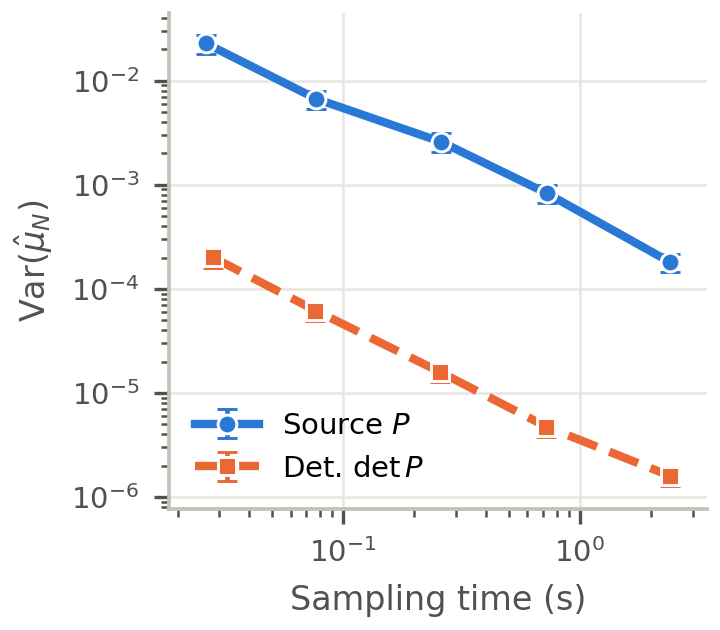
\includegraphics[width=\linewidth]{../results/estimator-variance/hmm.png}
        \caption{\texttt{hmm}: $113\times$ lower}
        \label{fig:estimator-variance-hmm}
    \end{subfigure}
    \hfill
    \begin{subfigure}[t]{0.32\linewidth}
        \centering
        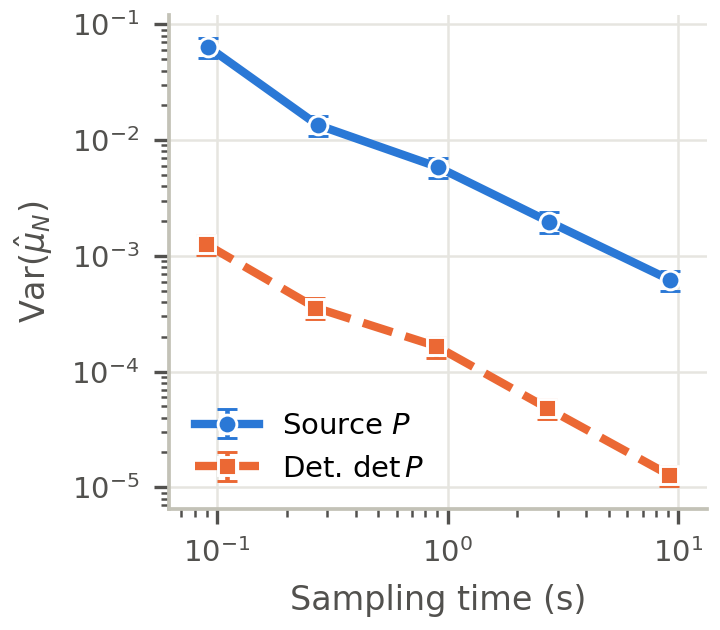
\includegraphics[width=\linewidth]{../results/estimator-variance/load.png}
        \caption{\texttt{load}: $48.4\times$ lower}
        \label{fig:estimator-variance-load}
    \end{subfigure}
    \caption{Empirical estimator variance $\operatorname{Var}(\hat{\mu}_N)$ versus mean sampling time for the
    source program $P$ and its determinization $\det P$, on log--log axes. Each point is a sample size
    $N \in \{10^3, 3 \cdot 10^3, 10^4, 3 \cdot 10^4, 10^5\}$; the estimator variance is the variance of the
    Monte Carlo estimates across 50 independent replicates, with error bars showing $\pm 1$ standard error. Subcaptions give the reduction in estimator
    variance at $N = 10^5$.}
    \label{fig:estimator-variance-vs-time}
\end{figure}